\begin{table}[h!]
\resizebox{\columnwidth}{!}{%
\begin{tabular}{lr}
\toprule
h & Q \\
\midrule
$0.140 \pm 0.010$ & 0.00 \\
$0.160 \pm 0.010$ & 0.00 \\
$0.180 \pm 0.010$ & 0.00 \\
$0.190 \pm 0.010$ & 0.00 \\
$0.150 \pm 0.010$ & 0.00 \\
$0.190 \pm 0.010$ & 0.00 \\
\bottomrule
\end{tabular}

}
\caption{Table of $R^2$ score and calculated unknown flowrate for each material and axis}
\label{table:results}
\end{table}
As seen in Table \ref{table:results} it is clear, that $axis = 0$ is the best axis to apply our model from eq. \ref{eq:linfunc} on. This is done in figure \ref{fig:copper}, \ref{fig:galvanized} and \ref{fig:PVC}, from which the unknown flow rates are determined, as described in section \ref{sec_level1}. It is also clear from some of the flow rates, some having very large uncertainties and one even being negative.


\begin{figure}[h!]
    \centering
    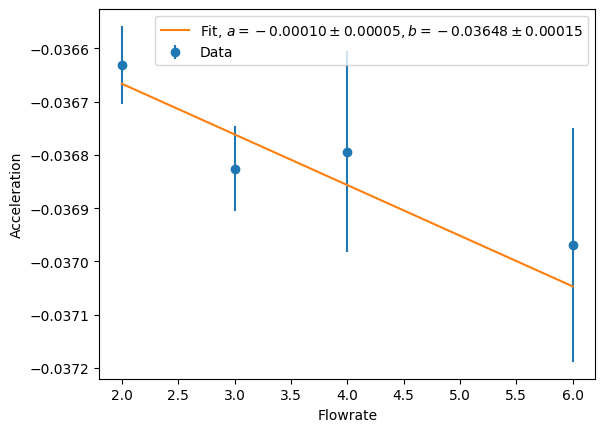
\includegraphics[width=55mm]
    {Python/Lab6/Plots/copper_axis0.png}
    \caption{Copper} 
    \label{fig:copper}
\end{figure}

\begin{figure}[h!]
    \centering
    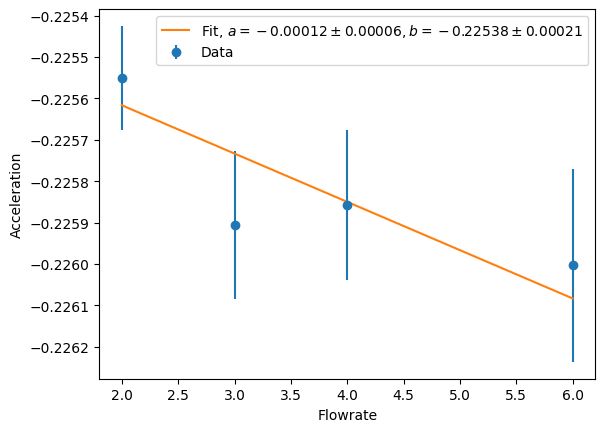
\includegraphics[width=55mm]
    {Python/Lab6/Plots/galvanized_axis0.png}
    \caption{Galvanized} 
    \label{fig:galvanized}
\end{figure}
  
\begin{figure}[h!]
    \centering
    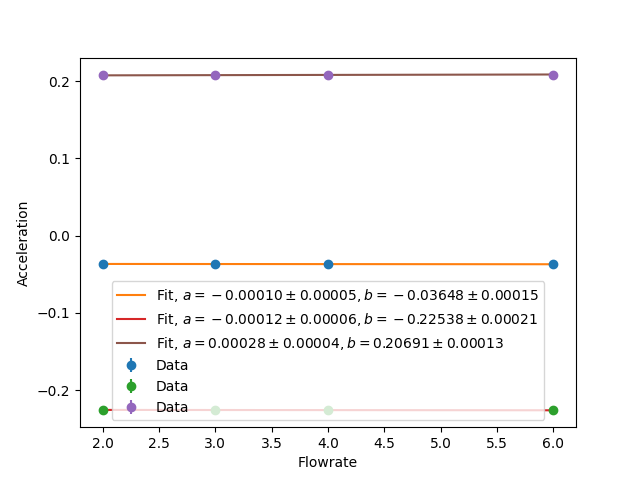
\includegraphics[width=55mm]
    {Python/Lab6/Plots/pvc_axis0.png}
    \caption{PVC} 
    \label{fig:PVC}
\end{figure}

  





